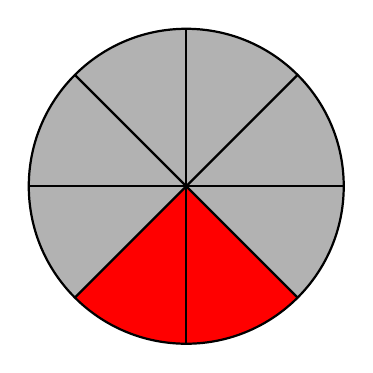
\begin{tikzpicture}

\def\R{2} % Raio da pizza

% Desenha as fatias
\foreach \i in {0,...,7} {
  \pgfmathsetmacro{\start}{\i*45}
  \pgfmathsetmacro{\end}{(\i+1)*45}
  % Cor vermelha para as duas últimas fatias (posição 5 e 6)
  \ifnum\i=5
    \fill[red] (0,0) -- (\start:\R) arc (\start:\end:\R) -- cycle;
  \else\ifnum\i=6
    \fill[red] (0,0) -- (\start:\R) arc (\start:\end:\R) -- cycle;
  \else
    \fill[gray!60] (0,0) -- (\start:\R) arc (\start:\end:\R) -- cycle;
  \fi\fi
}

% Contorno do círculo
\draw[thick] (0,0) circle (\R);

% Linhas divisórias
\foreach \a in {0,45,...,315} {
  \draw[thick] (0,0) -- (\a:\R);
}

\end{tikzpicture}